\documentclass[10pt]{article}


\usepackage{fullpage}
\usepackage{graphicx}
\usepackage{caption}
\usepackage{subcaption}

\begin{document}

\title{MIMIC2V30 SAPS-I}
\maketitle

\noindent SAPS-I variables were collected using begin and end 
time of ICU stay days (using ICUSTAY\_DAYS tables) 
for all days longer than 12 hours. The first, maximum, and minimum SAPS-I 
were calculated from all the SAPS-I values over the duratinon of the ICU 
stay. The complete list of SAPS-I variables include:
\begin{itemize}
\item {\bf Age} 
\item {\bf Temperature} itemid in (676, 677, 678, 679, 227054, 223762, 223761), range 15 - 45 
\item {\bf Heart Rate} itemid in (220045, 211), range 10 - 250
\item {\bf Systolic BP} itemid in (51, 455, 225309, 2293), range 20 - 300
\item {\bf HCT} itemid in (50383,50029), range 5 - 100
\item {\bf WBC} itemid in (51326,50468,50316), range  5 - 2,000,000
\item {\bf Glucose} itemid in (50112,50936,50006), range 0.5 - 1000
\item {\bf HCO3} itemid in (50803,50022,50172,50025), range  2 - 100
\item {\bf Potassium} itemid in (50009,50821,50976,50149), range 0.5 - 70
\item {\bf Sodium} itemid in (50989,50823,50159,50012), range 50 - 300
\item {\bf Creatinine} itemid in (50090,50916), range 0 - 30
\item {\bf BUN} itemid in (781,225624,1162,3737,227000,5876,227001), range 1 - 100
\item {\bf Glasgow Coma Score} itemid in (227013,198,226755), range 2 - 15
\item {\bf Urine Output} 
\end{itemize}
Sum over itemid in (40056, 40057, 40058, 40070, 40086, 40095, 40097, 40406,
      40429, 40474, 40535, 40652, 40716, 41923, 42367, 42508, 42511, 42677,
      42811, 42860, 43054, 46181)
\begin{itemize}
\item {\bf Mechanical Ventilation} 
\item {\bf Spont.~Resp.~Rate} itemid in (220210,618,653,3603,219,1635,8113,1884,615), range 2 - 80
\end{itemize}

\begin{figure}
\centering 
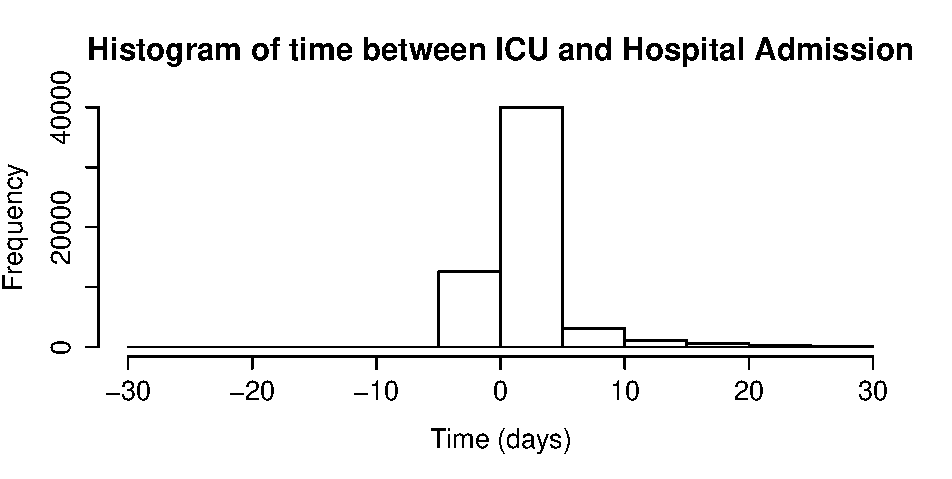
\includegraphics[width=0.8\linewidth]{../../figure/hist_hadm_dt.pdf}
\end{figure}


\begin{figure}
\centering
        \begin{subfigure}[b]{0.5\textwidth}
          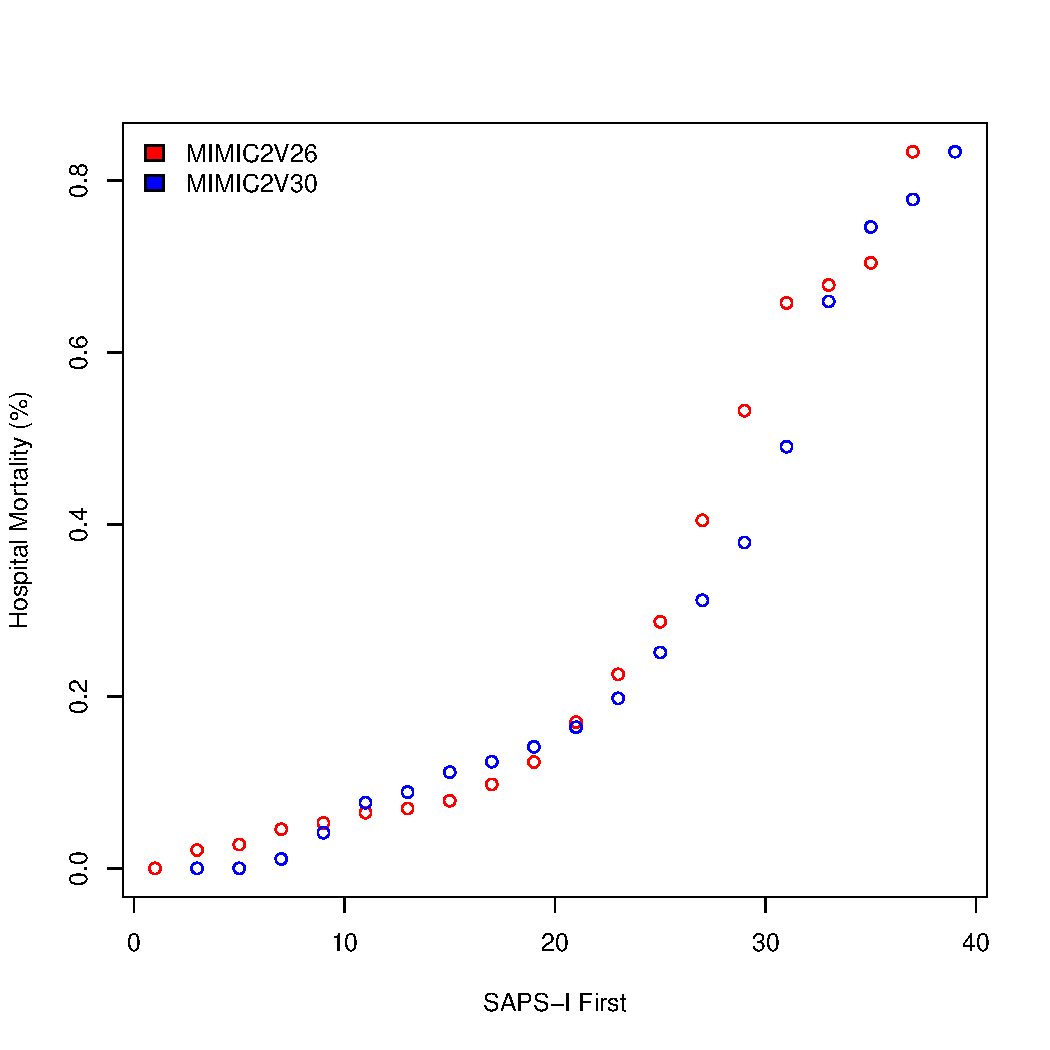
\includegraphics[width=\linewidth]{../../figure/fig_sapsi_mort.pdf}
        \end{subfigure}%
        \begin{subfigure}[b]{0.5\textwidth}
          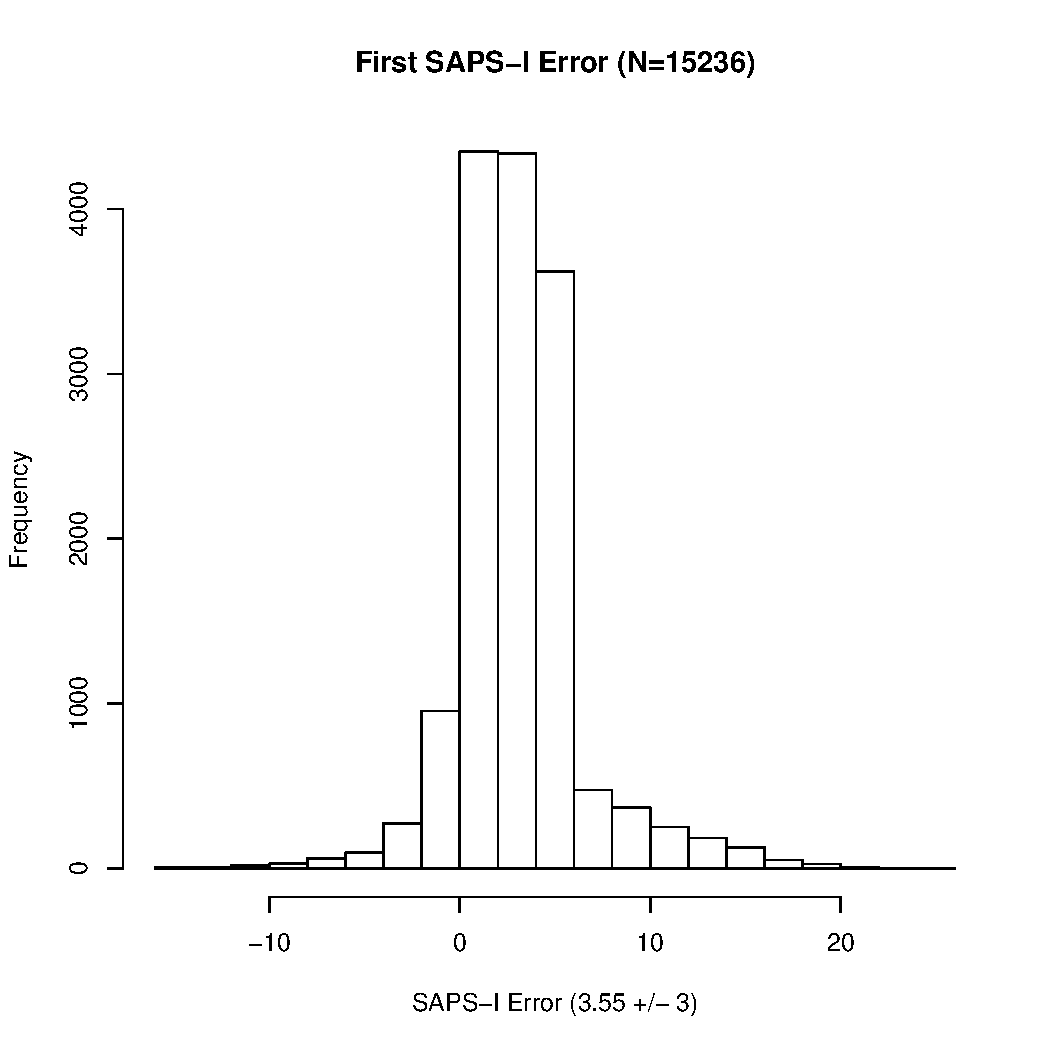
\includegraphics[width=\linewidth]{../../figure/fig_hist_sapsi_first_err.pdf}
        \end{subfigure}

\end{figure}

\begin{figure}
\centering
        \begin{subfigure}[b]{0.5\textwidth}
                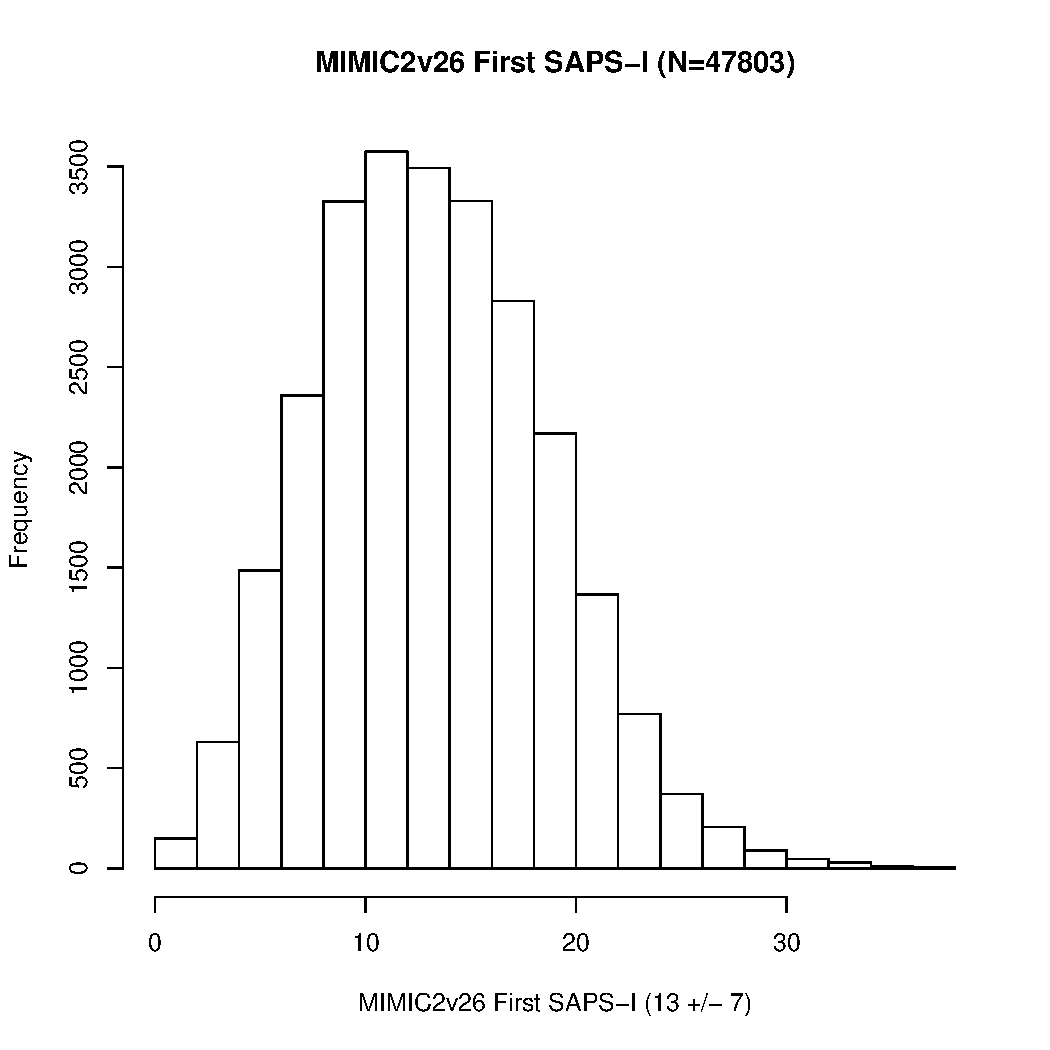
\includegraphics[width=\linewidth]{../../figure/fig_hist_sapsi_first_mimic2v26.pdf}
        \end{subfigure}%
        \begin{subfigure}[b]{0.5\textwidth}
                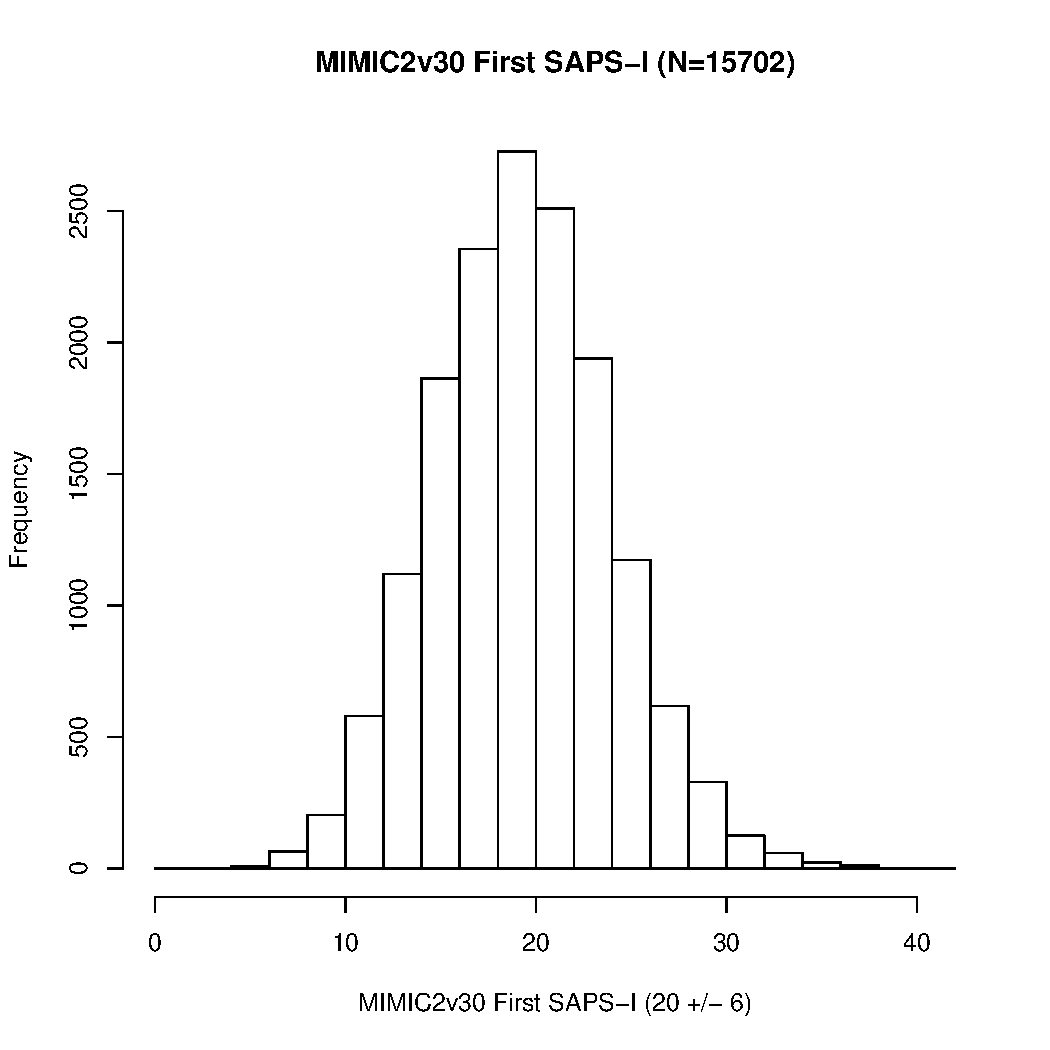
\includegraphics[width=\linewidth]{../../figure/fig_hist_sapsi_first_mimic2v30.pdf}
        \end{subfigure}
\end{figure}

\begin{figure}
\centering
        \begin{subfigure}[b]{0.5\textwidth}
          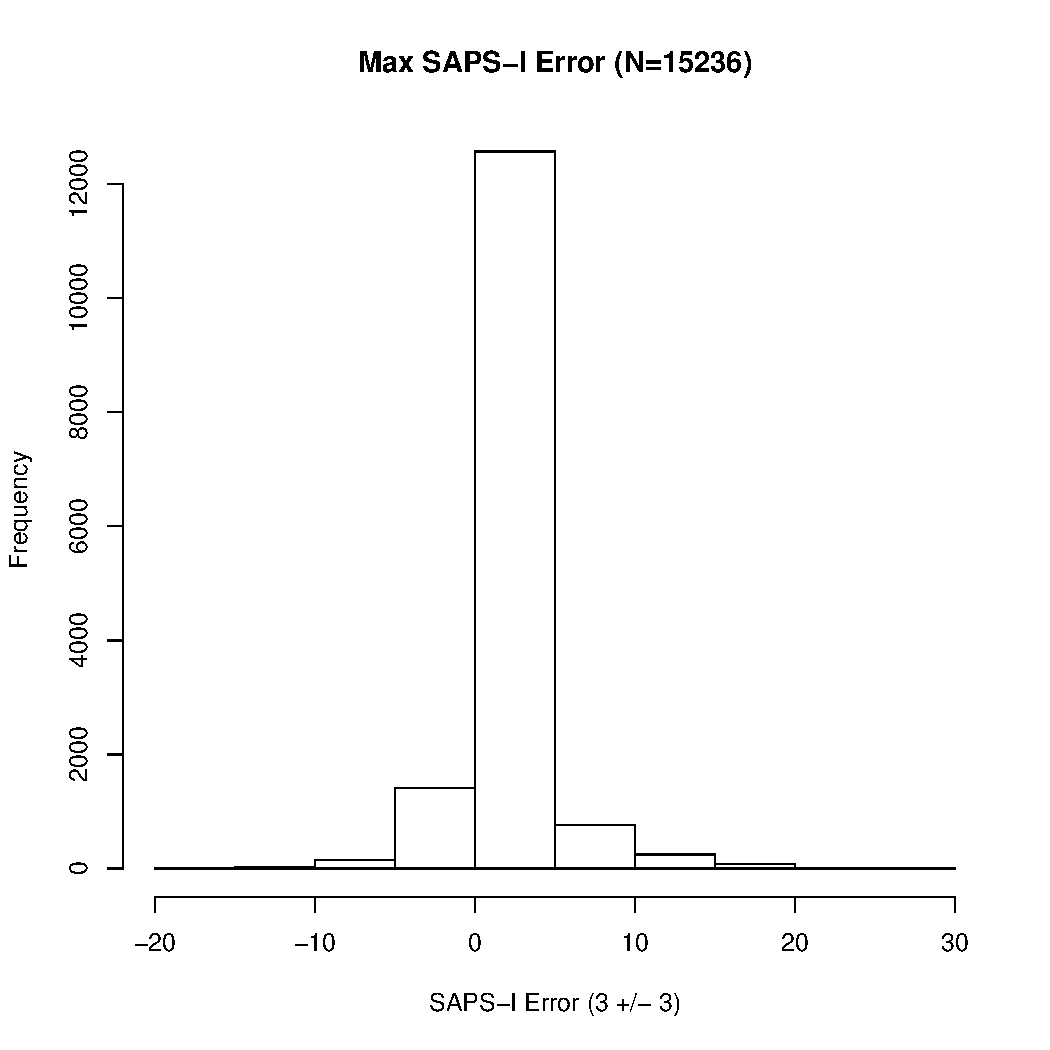
\includegraphics[width=\linewidth]{../../figure/fig_hist_sapsi_max_err.pdf}
        \end{subfigure}%
        \begin{subfigure}[b]{0.5\textwidth}
          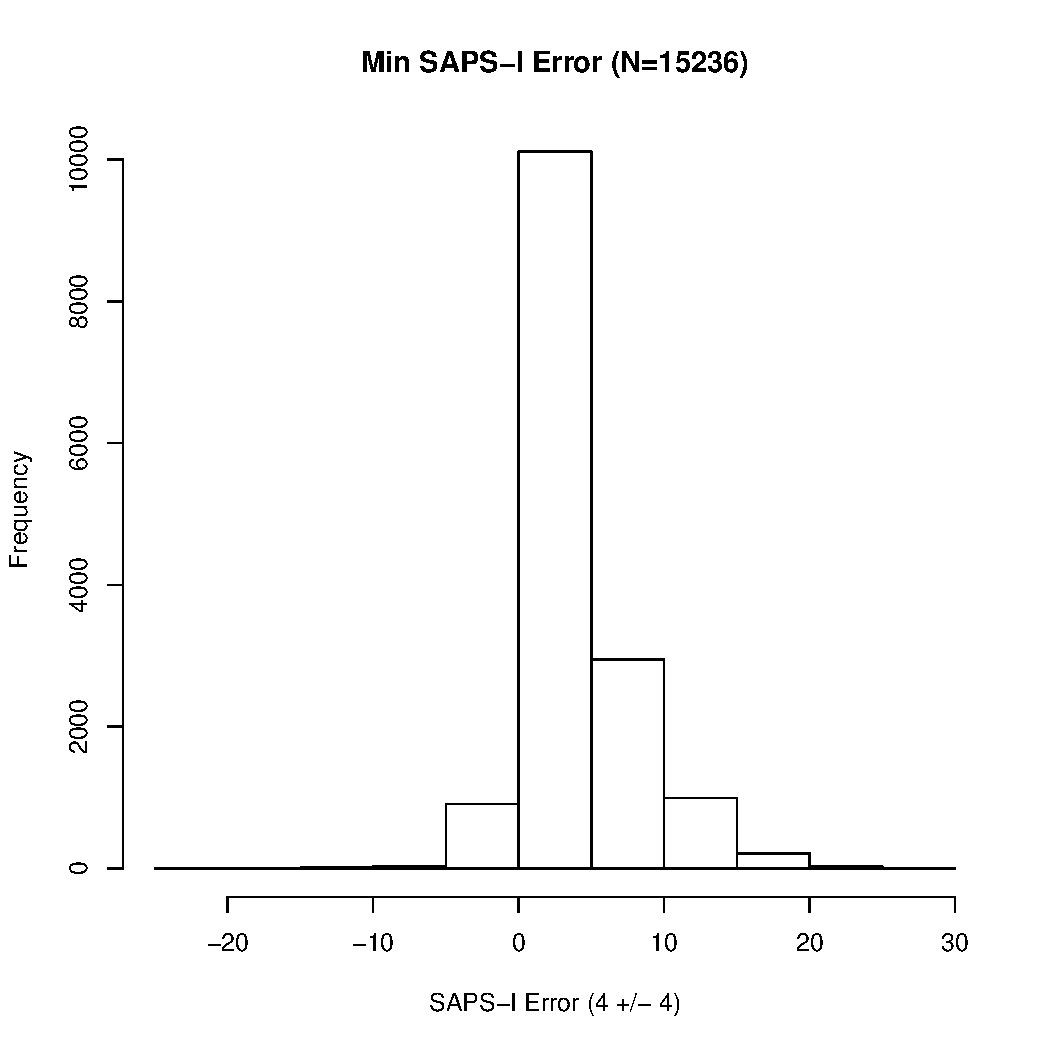
\includegraphics[width=\linewidth]{../../figure/fig_hist_sapsi_min_err.pdf}
        \end{subfigure}
\end{figure}

\begin{figure}
        \begin{subfigure}[b]{0.5\textwidth}
                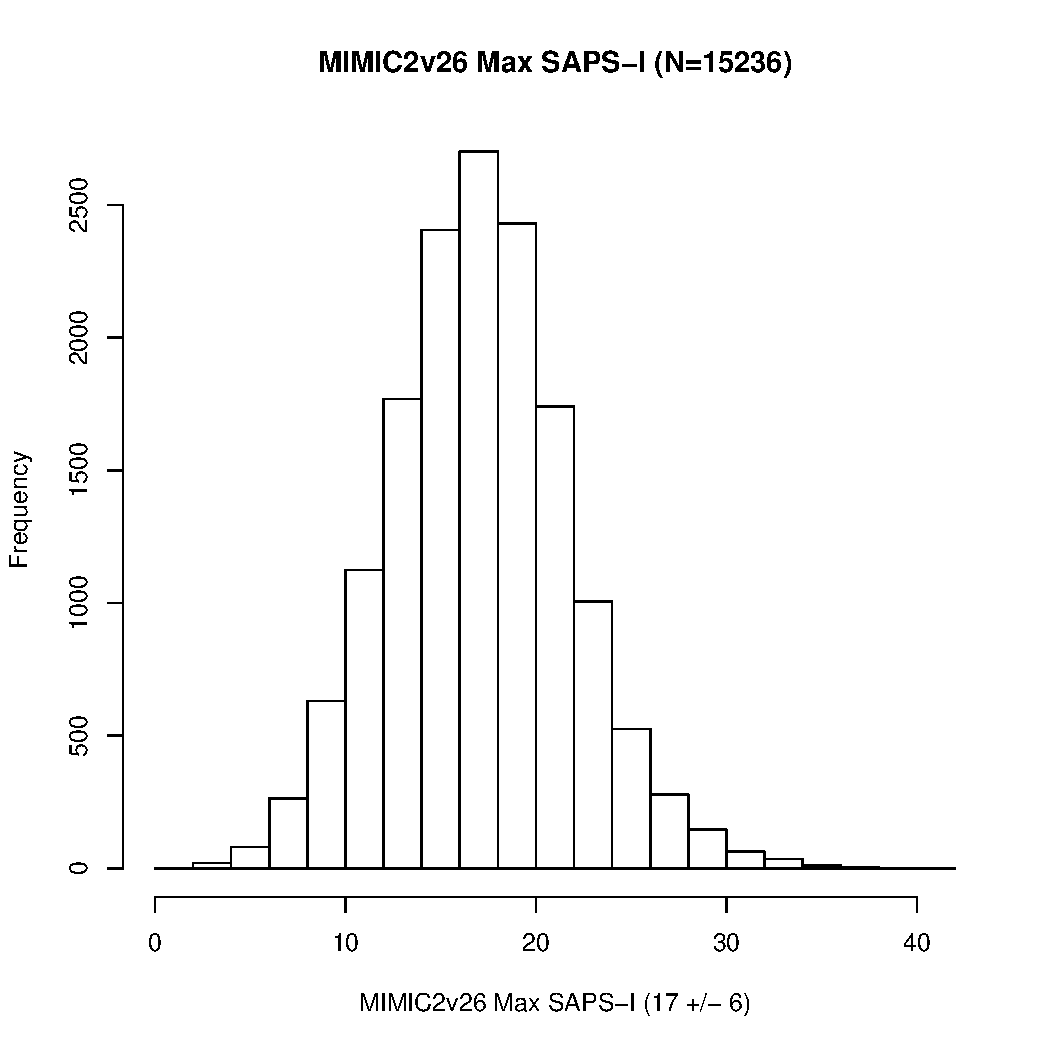
\includegraphics[width=\linewidth]{../../figure/fig_hist_sapsi_max_mimic2v26.pdf}
        \end{subfigure}%
        \begin{subfigure}[b]{0.5\textwidth}
                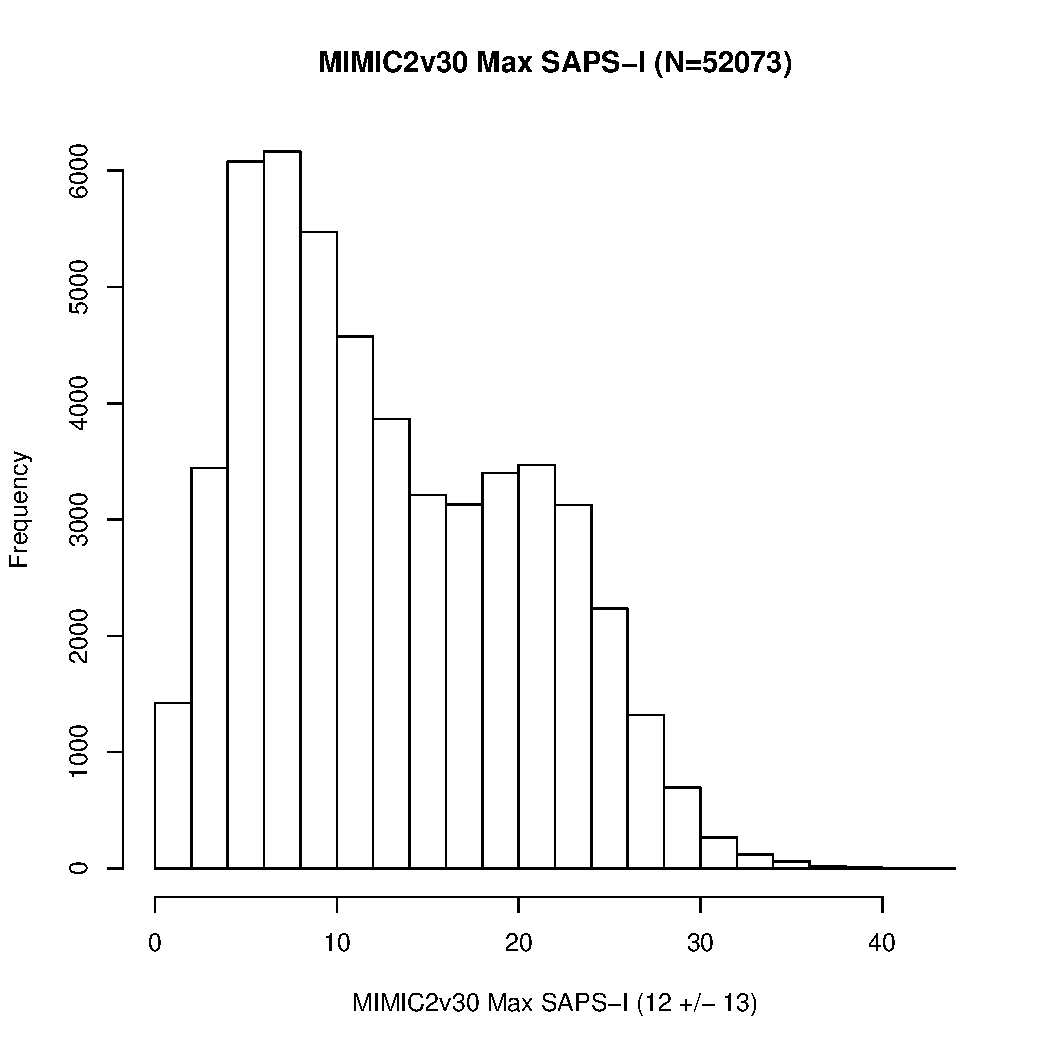
\includegraphics[width=\linewidth]{../../figure/fig_hist_sapsi_max_mimic2v30.pdf}   
        \end{subfigure}
\end{figure}

\begin{figure}
        \begin{subfigure}[b]{0.5\textwidth}
                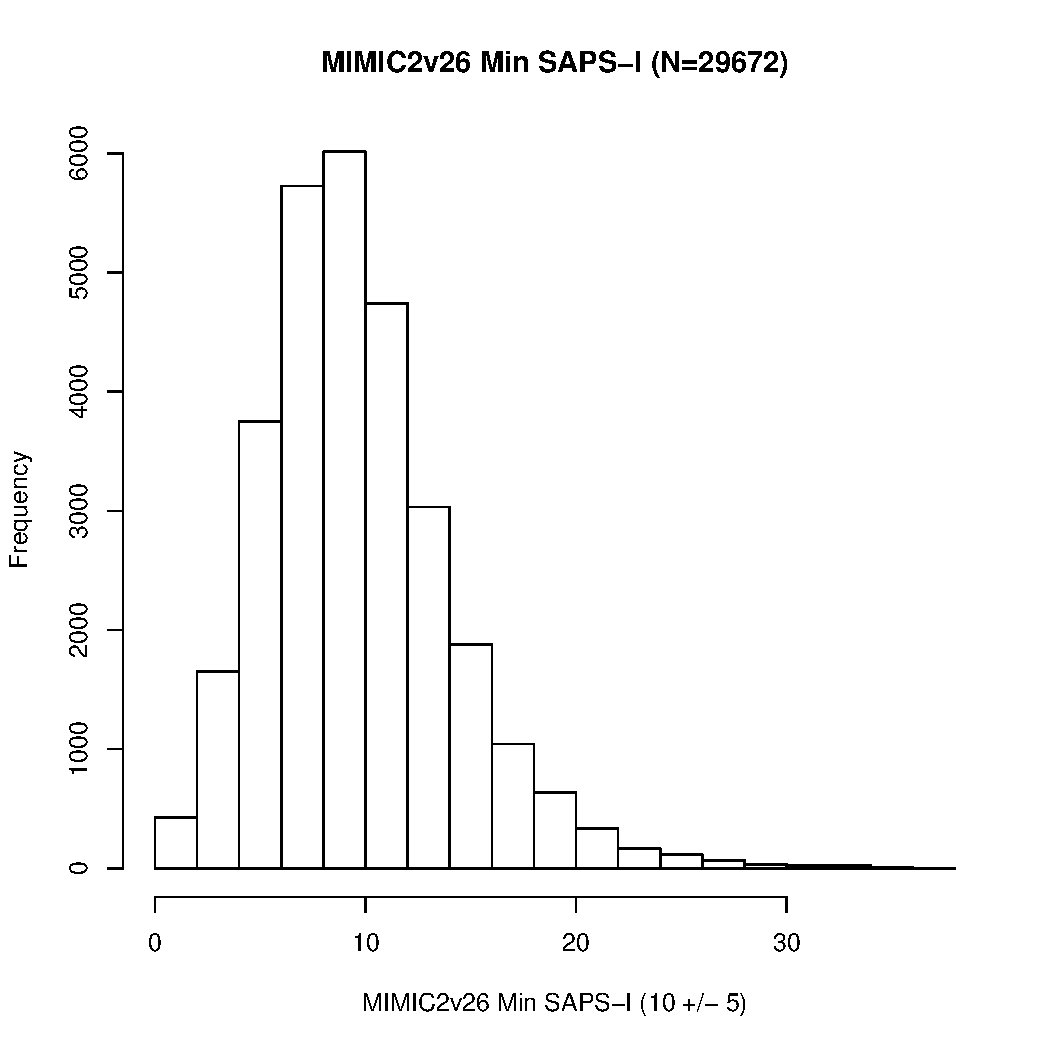
\includegraphics[width=\linewidth]{../../figure/fig_hist_sapsi_min_mimic2v26.pdf}
        \end{subfigure}%
        \begin{subfigure}[b]{0.5\textwidth}
                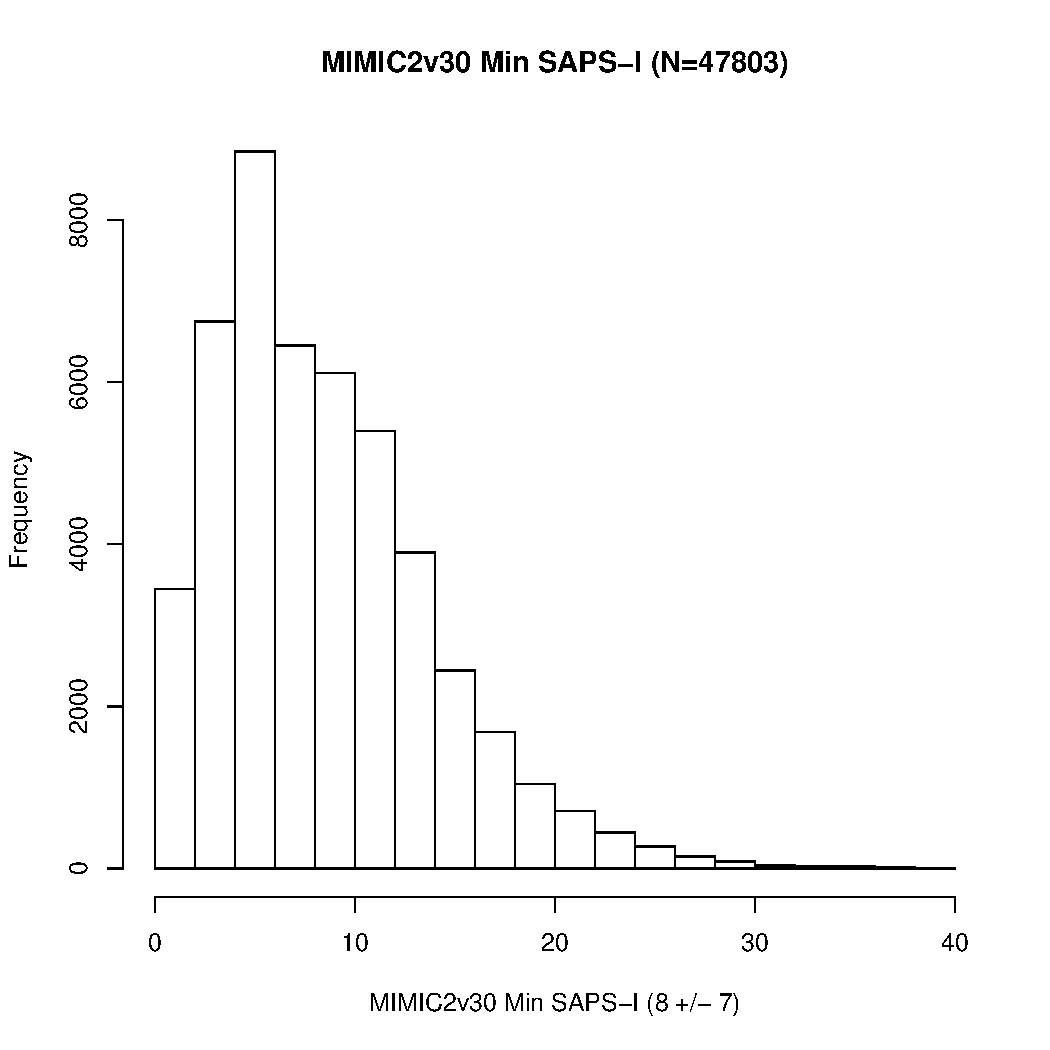
\includegraphics[width=\linewidth]{../../figure/fig_hist_sapsi_min_mimic2v30.pdf}
        \end{subfigure}
\end{figure}




\end{document}
